% Household mechanisms: all numerical panels use the same post-interest,
% no-Estate-A chain-13 reference at fixed prices. Reproduction and exact
% experiment definitions: output/model/credit_mechanism_20261004/mechanism_slides/README.md.

\begin{frame}[t,label=mechanism-households]{Household Choices at First Birth}
\small
Initially childless renters, ages 22--25, at the middle earnings state.
\begin{center}
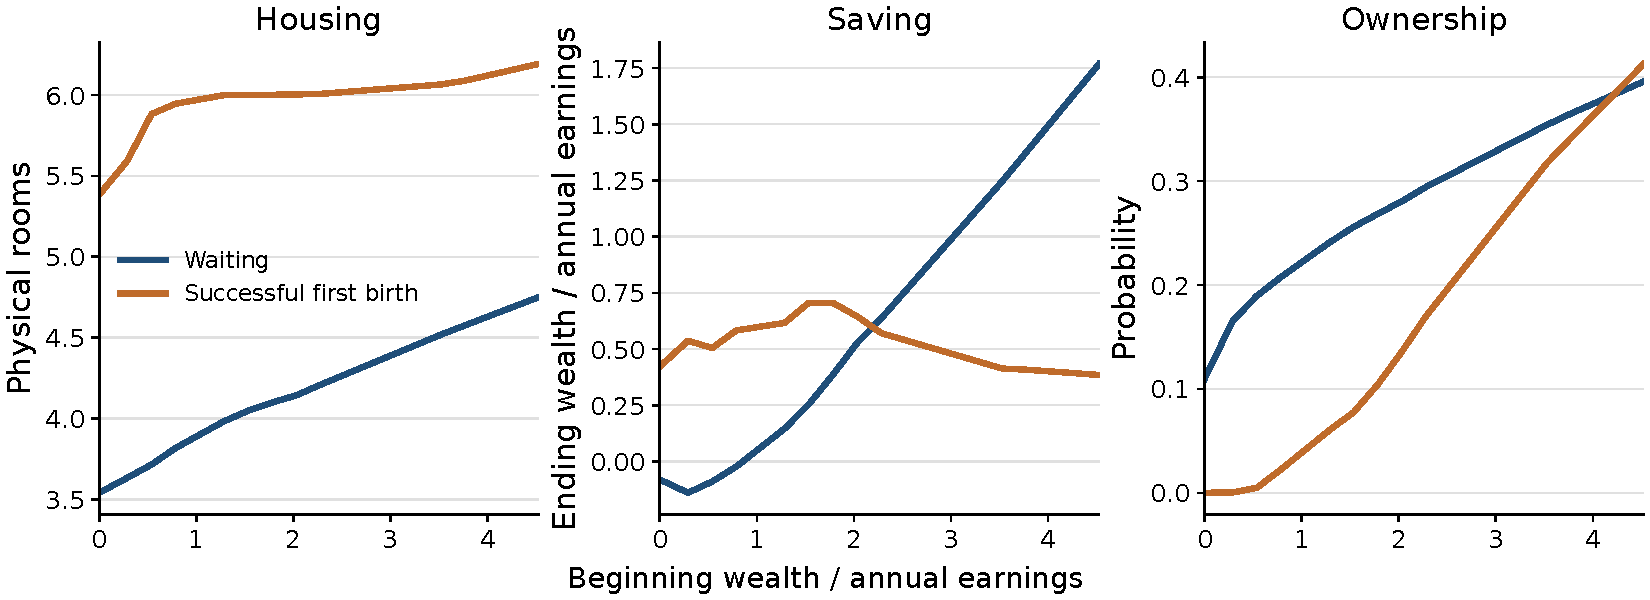
\includegraphics[width=\textwidth,height=0.66\textheight,keepaspectratio]{JMP_slides/mechanisms/figures/household_policies.pdf}
\end{center}
\vfill
A first child raises space demand; at low wealth, households rent and retain more liquid assets.
\end{frame}

\begin{frame}[t,label=mechanism-floor]{The Parenthood Space Requirement}
\small
Initially childless renters, ages 22--25, middle earnings state.\\
Raise required space from $2.594$ to $2.781$ rooms; prices and other inputs stay fixed.
\begin{center}
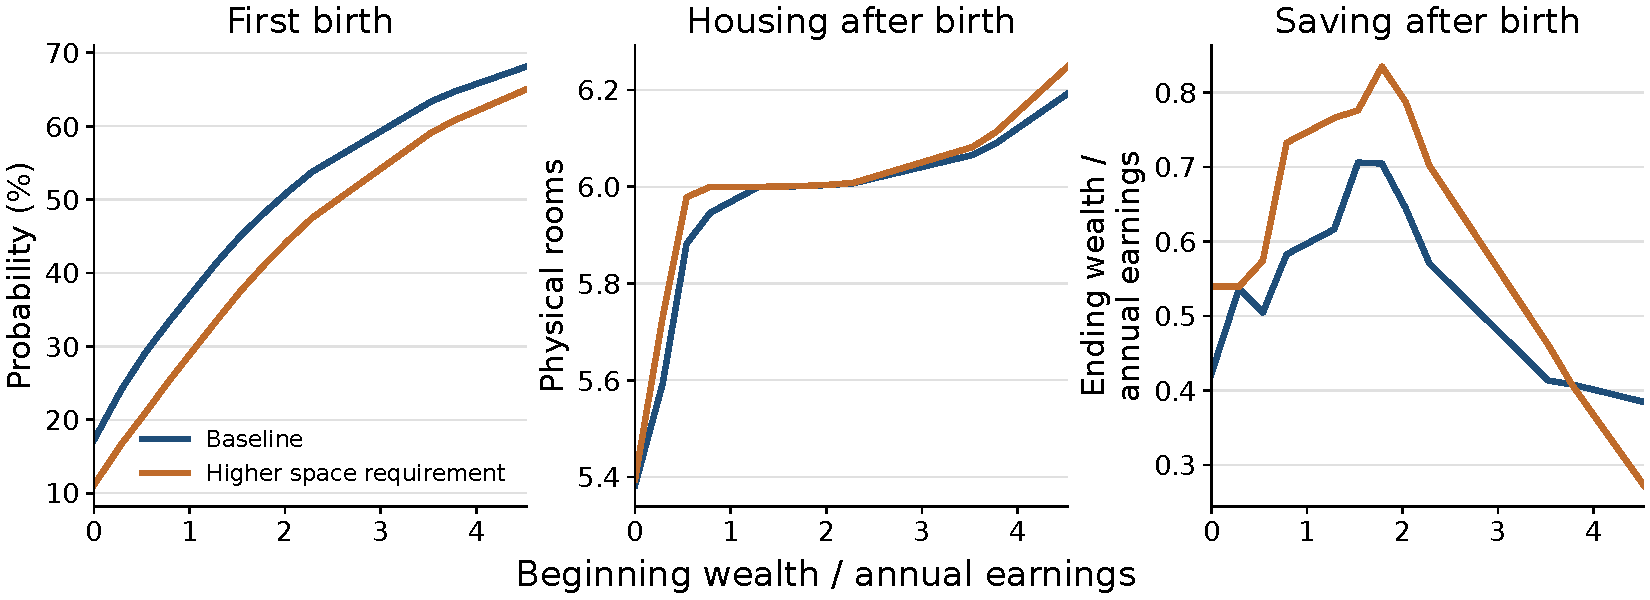
\includegraphics[width=\textwidth,height=0.58\textheight,keepaspectratio]{JMP_slides/mechanisms/figures/parenthood_floor.pdf}
\end{center}
\vfill
Requiring more space reduces first-birth probabilities at the same household resources.
\end{frame}

\begin{frame}[t,label=mechanism-price]{Housing Costs and Fertility}
\small
Impose a $10\%$ increase in house prices and rents; evaluate households at the same initial states.
\begin{center}
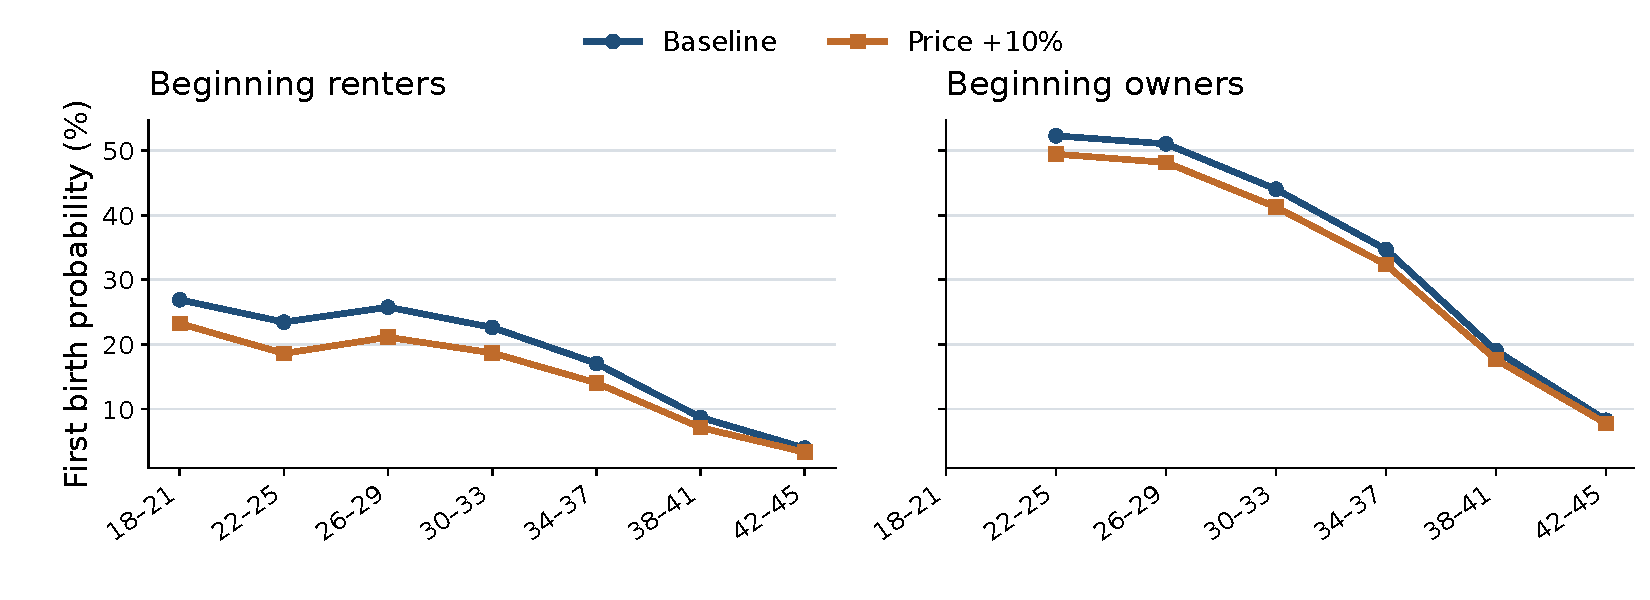
\includegraphics[width=\textwidth,height=0.66\textheight,keepaspectratio]{JMP_slides/mechanisms/figures/first_birth_price110_by_beginning_tenure.pdf}
\end{center}
\vfill
Birth probabilities fall, with a larger response among households that start as renters.
\end{frame}

\begin{frame}[t,label=mechanism-credit]{Mortgage Finance and Fertility}
\small
Increase the financed share from $80\%$ to $95\%$, holding house prices and rents fixed.
\begin{center}
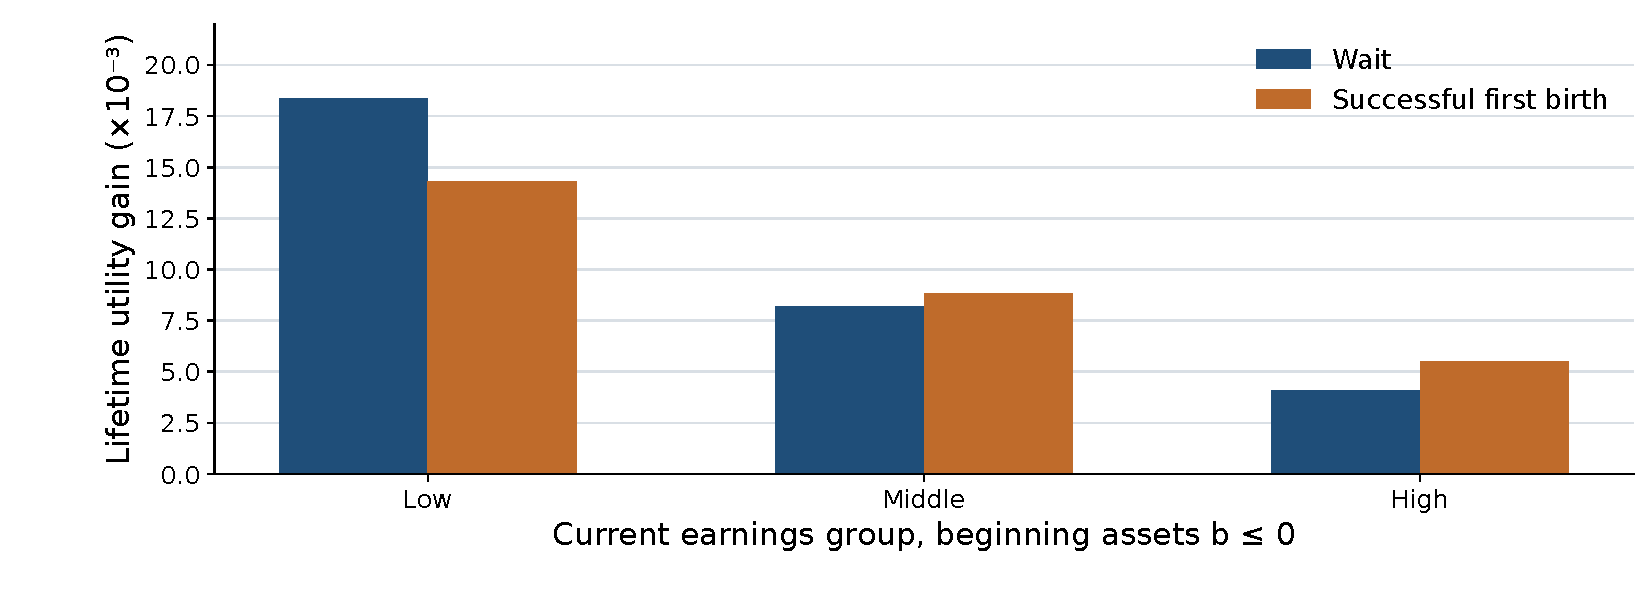
\includegraphics[width=\textwidth,height=0.55\textheight,keepaspectratio]{JMP_slides/mechanisms/figures/credit_phi095_wait_success_gains_debt_states.pdf}
\end{center}
{\scriptsize Value gains where both choices have positive probability: $92.5\%$ of low-earner exposure.}
\vfill
Credit helps both choices; fertility depends on the gain from a child relative to waiting.\\[2pt]
{\footnotesize Across the lifecycle: young ownership $+10.1$ percentage points; birth flows $-0.25\%$.}
\end{frame}

\begin{frame}[t,label=mechanism-rentals]{Rental Space and Homeownership}
\small
Change the maximum size of rental housing, holding prices and other inputs fixed.
\begin{center}
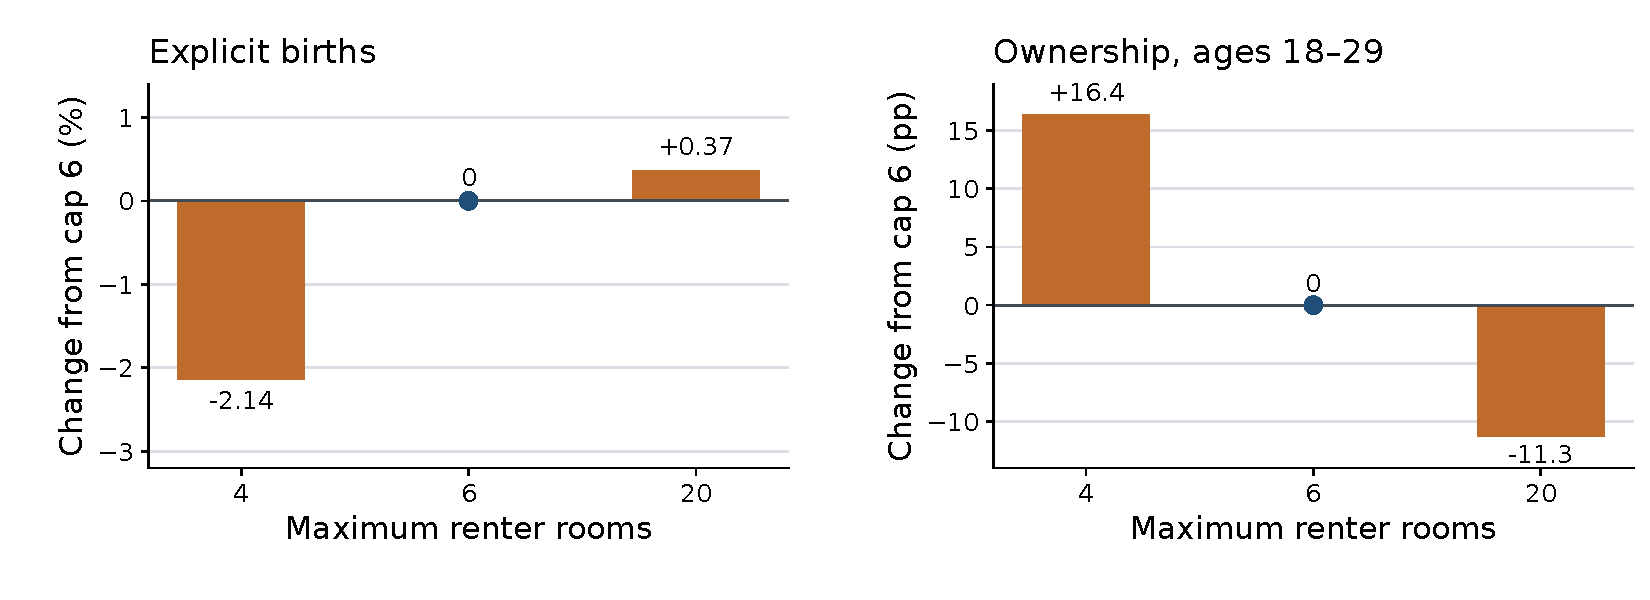
\includegraphics[width=\textwidth,height=0.66\textheight,keepaspectratio]{JMP_slides/mechanisms/figures/renter_room_cap_births_ownership.pdf}
\end{center}
\vfill
Larger rentals substitute for ownership, while birth flows change little.
\end{frame}
